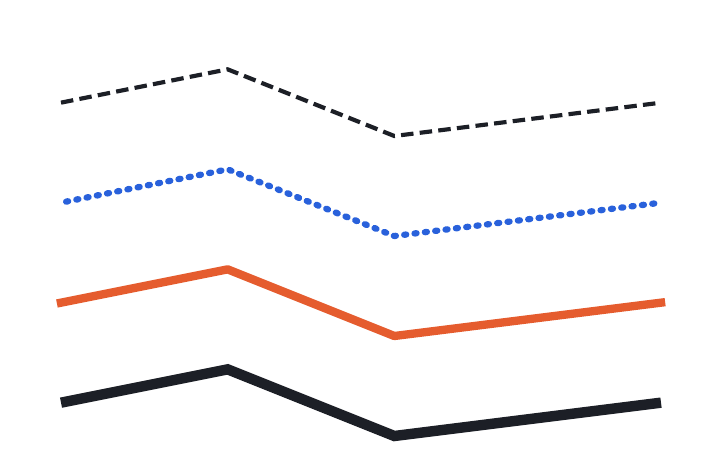
\begin{tikzpicture}[every node/.style={inner sep=0bp,outer sep=0bp}]
  \definecolor{qcA}{rgb}{0.11,0.12,0.15}
  \definecolor{qcB}{rgb}{0.16,0.38,0.86}
  \definecolor{qcC}{rgb}{0.9,0.36,0.18}
  \useasboundingbox (0bp,0bp) rectangle (240bp,150bp);
  \path[draw=qcA,line width=1.5bp,dash pattern=on 4.5bp off 2.25bp] (12bp,123bp) -- (72bp,135bp) -- (132bp,111bp) -- (228bp,123bp);
  \path[draw=qcB,line width=2.25bp,dash pattern=on 0.75bp off 3bp,dash phase=1.875bp,line cap=round,line join=round] (12bp,87bp) -- (72bp,99bp) -- (132bp,75bp) -- (228bp,87bp);
  \path[draw=qcC,line width=3bp,dash pattern=on 7.5bp off 1.5bp on 1.5bp off 1.5bp,dash phase=0.75bp,line cap=rect,line join=bevel] (12bp,51bp) -- (72bp,63bp) -- (132bp,39bp) -- (228bp,51bp);
  \path[draw=qcA,line width=3.75bp,miter limit=1.5] (12bp,15bp) -- (72bp,27bp) -- (132bp,3bp) -- (228bp,15bp);
\end{tikzpicture}
